%%%%%%%%%%%%%%%%%%%%%%%%%%%%%%%%%%%%%%%%%
% Seminário
% LaTeX Template
% Version 1.0 (13/03/19)
%
% Author: Fred Guth (fredguth@fredguth.com)
%
% License:
% CC BY-NC-SA 3.0 (http://creativecommons.org/licenses/by-nc-sa/3.0/)
%
%%%%%%%%%%%%%%%%%%%%%%%%%%%%%%%%%%%%%%%%%

%----------------------------------------------------------------------------------------
%	PACKAGES AND OTHER DOCUMENT CONFIGURATIONS
%----------------------------------------------------------------------------------------

\documentclass[
10pt, % Default font size is 10pt, can alternatively be 11pt or 12pt
a4paper, % Alternatively letterpaper for US letter
onecolumn, % Alternatively twocolumn
% portrait % Alternatively landscape
]{article}

%%%%%%%%%%%%%%%%%%%%%%%%%%%%%%%%%%%%%%%%%
% Paper Notes
% Structure Specification File
% Version 1.0 (25/10/18)
%
% Author: Fred Guth (fredguth@fredguth.com
%
% License:
% CC BY-NC-SA 3.0 (http://creativecommons.org/licenses/by-nc-sa/3.0/)
%
%%%%%%%%%%%%%%%%%%%%%%%%%%%%%%%%%%%%%%%%%%%%%%%%%%%%%%%%%%%%%%%%%%%%%%%%%%%%%%%%%%

%----------------------------------------------------------------------------------------
%	REQUIRED PACKAGES
%----------------------------------------------------------------------------------------

\usepackage[includeheadfoot,columnsep=2cm, left=1in, right=1in, top=.5in, bottom=.5in]{geometry} % Margins

\usepackage[utf8]{inputenc}
\usepackage{XCharter} % XCharter as the main font
\usepackage{booktabs}
\usepackage{natbib} % Use natbib to manage the reference
\usepackage{bibentry}
\usepackage{amsmath}
\usepackage{amsthm}
\usepackage{graphicx, wrapfig}
\graphicspath{ {./imgs/} }

\nobibliography*
\bibliographystyle{plain} % Citation style

\usepackage[brazil]{babel} % Use english by default

%----------------------------------------------------------------------------------------
%	CUSTOM COMMANDS
%----------------------------------------------------------------------------------------
\newcommand{\horrule}[1]{\rule{\linewidth}{#1}} % Create horizontal rule command with 1 argument of height
\newcommand{\papertitle}[1]{\renewcommand{\papertitle}{#1}} % Define a command for storing the article title
\newcommand{\papercitation}[1]{\renewcommand{\papercitation}{#1}} % Define a command for storing the article citation
\newcommand{\lectureabstract}[1]{\renewcommand{\lectureabstract}{#1}}
% \newcommand{\doctitle}{``\papertitle''\---\papercitation  } % Define a command to store the article information as it will appear in the title and header

\newcommand{\datenotesstarted}[1]{\renewcommand{\datenotesstarted}{#1}} % Define a command to store the date when notes were first made
\newcommand{\docdate}[1]{\renewcommand{\docdate}{#1}} % Define a command to store the date line in the title

\newcommand{\docauthor}[1]{\renewcommand{\docauthor}{#1}} % Define a command for storing the article notes author

% Define a command for the structure of the document title
\newcommand{\printtitle}{

\begin{center}

  \horrule{0.5pt} \\[0.4cm] % Thin top horizontal rule

  \bigskip

  \textbf{\Large{"\papertitle"}}
  
  \bigskip
  \begin{minipage}{.9\textwidth}
  \lectureabstract
  \end{minipage}
  \bigskip
  
  \docdate

  \docauthor

  \bigskip
  

  \horrule{2pt} \\[0.5cm] % Thick bottom horizontal rule

\end{center}


}

%----------------------------------------------------------------------------------------
%	STRUCTURE MODIFICATIONS
%----------------------------------------------------------------------------------------

\setlength{\parskip}{3pt} % Slightly increase spacing between paragraphs

% Uncomment to center section titles
%\usepackage{sectsty}
%\sectionfont{\centering}

% Uncomment for Roman numerals for section numbers
%\renewcommand\thesection{\Roman{section}}
 % Input the file specifying the document layout and structure
%----------------------------------------------------------------------------------------
%	ARTICLE INFORMATION
%----------------------------------------------------------------------------------------

\papertitle{Uma Brevíssima Introdução à \\  Teoria da Aprendizagem Computacional} % The title of the article
\lectureabstract{Teoria de Aprendizagem Computacional é o ramo de estudo que objetiva aplicar Teoria da Complexidade para problemas de aprendizado. Nesta breve introdução, iremos apresentar, de forma intuitiva, o Modelo de Aprendizado-PAC (\emph{Probably Approximately Correct}) de Leslie Valiant (1984) que é o trabalho seminal da área. }
\datenotesstarted{12 de março de 2019} % The date when these notes were first made
\docdate{\datenotesstarted; rev. \today} % The date when the notes were lasted updated (automatically the current date)

\docauthor{Fred Guth} % Your name
\newcommand*\rfrac[2]{{}^{#1}\!/_{#2}}
%----------------------------------------------------------------------------------------

\begin{document}

\pagestyle{myheadings} % Use custom headers
\markright{\papertitle} % Place the article information into the header

%----------------------------------------------------------------------------------------
%	PRINT ARTICLE INFORMATION
%----------------------------------------------------------------------------------------

\thispagestyle{plain} % Plain formatting on the first page

\printtitle % Print the title

%----------------------------------------------------------------------------------------
%	ARTICLE NOTES
%----------------------------------------------------------------------------------------

\section{Preâmbulo} 

\begin{wrapfigure}{R}{1.5in}
    \framebox{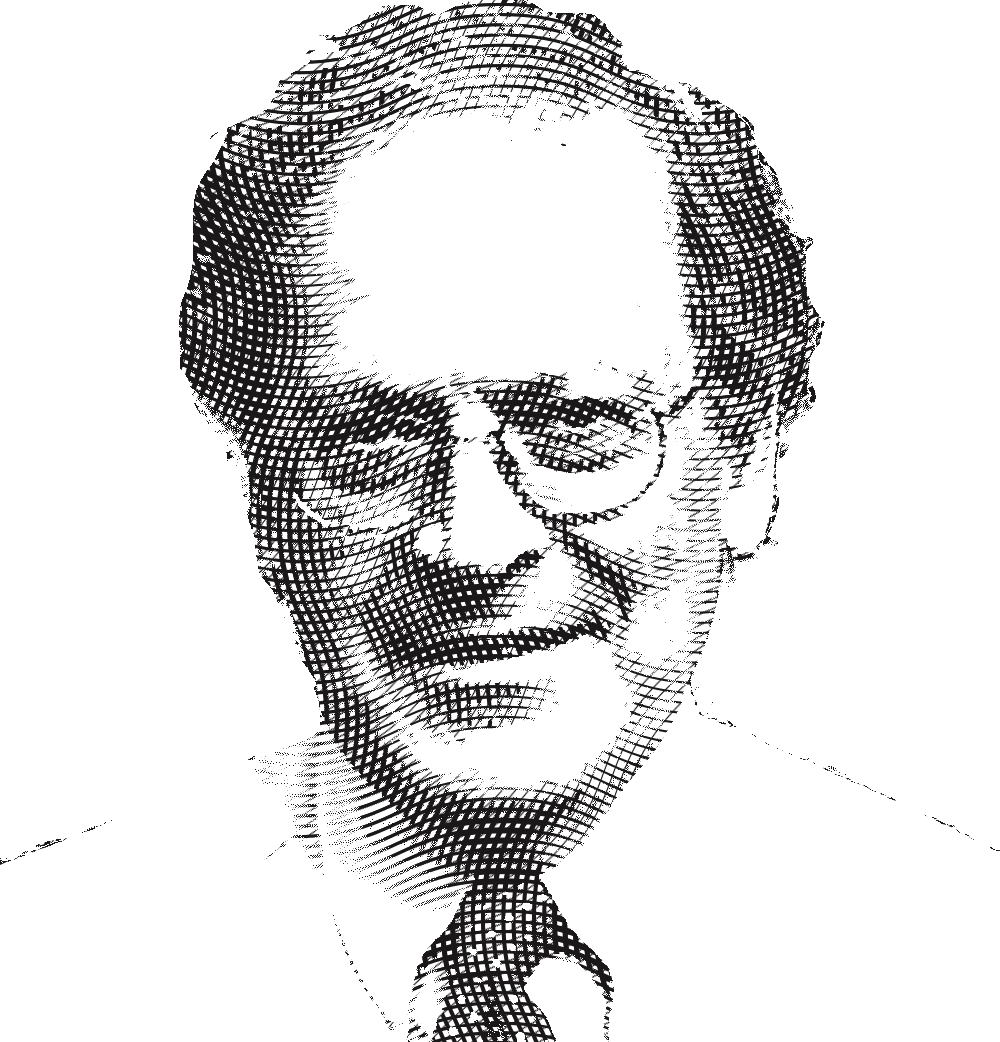
\includegraphics[width=1.5in]{leslie_bg2}}
    \caption{Leslie Valiant, Prêmio Turing 2010.}
    \label{leslie}
\end{wrapfigure}

Teoria da Complexidade Computacional, um dos alicerces da Ciência da Computação, tem por objetivo examinar e classificar problemas de acordo com suas dificuldades de solução. Ao estudar complexidade de algoritmos, entusiastas de aprendizado de máquina podem naturalmente se perguntar: \begin{quotation}Será que não seria possível analisar qual seria a quantidade de amostras necessárias para um algoritmo aprender uma tarefa?\end{quotation}
    
A resposta é sim. Em 1984, Leslie Valiant publicou o modelo de aprendizado \textbf{Provavelmente Aproximadamente Correto} (PAC, \emph{Probably Approximately Correct})\cite{Valiant1984}, justamente com o objetivo de incitar pesquisadores que estudavam complexidade de algoritmos a pensar problemas de aprendizado. 

Ele introduziu a ideia de problemas de aprendizado que são apreensíveis em tempo polinomial, \textbf{PAC apreensíveis}, em analogia com a classe dos problemas $P$. Pode-se dizer que foi bem sucedido:  diversos pesquisadores estenderam ou propuseram novas teorias, o que originou o ramo de estudo chamado de \textbf{Teoria de Aprendizado Computacional}, que tem até a sua própria conferência anual, COLT (\emph{Conference on Learning Theory})~\cite{COLT}.

Nesse trabalho, o objetivo é apresentar de forma intuitiva, reduzindo bastante os jargões, o Modelo de Aprendizado-PAC de Leslie Valiant que é o trabalho seminal da área. 

%------------------------------------------------

\section{O que é Apreensível?}
\begin{wrapfigure}{R}{1.5in}
    \framebox{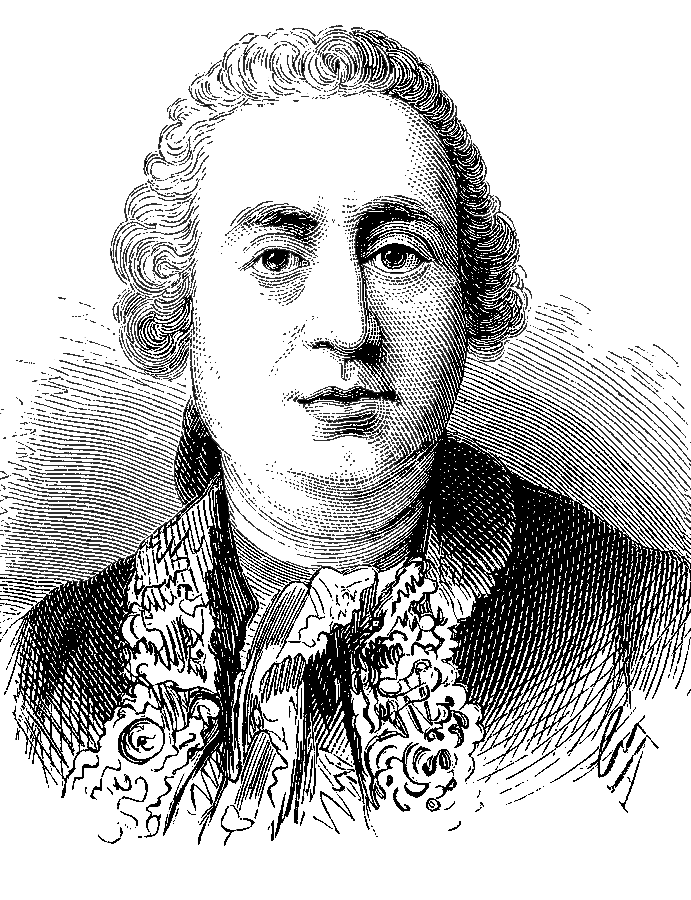
\includegraphics[width=1.5in]{hume_d2}}
    \caption{David Hume (1711-1776).}
    \label{hume}
\end{wrapfigure}

O que é apreensível? Essa é uma questão muito anterior à Ciência da Computação.  No século 18, o filósofo escocês David Hume se perguntou se é possível gerar conhecimento a partir da indução (\textbf{O problema da Indução})\cite{Hume2009Tratado}.  O que é justamente a base do aprendizado supervisionado, a área da Inteligência Artificial mais pesquisada no momento.

Para Hume, não há justificativa lógica para generalizações baseadas em indução. 
\begin{quotation}
    "O pão que comi anteriormente alimentou-me, (...) mas segue-se porventura disso outro pão deva igualmente alimentar-me em outra ocasião?  Essa ocasião não parece de nenhum modo necessária"~\cite{hume2004investigacoes}.
\end{quotation}
 Para ele nós vemos causalidade onde há apenas a conjunção constante entre dois acontecimentos distintos. Mas se isso é verdade, é possível obter conhecimento através da indução?  E se não é possível, o aprendizado indutivo supervisionado não tem justificativa? Pior, o método científico não pode ser logicamente justificado?

A abordagem de Valiant traz uma resposta ao mesmo tempo prática e formal para esse problema.  Não é possível dizer que "esse pão que ainda não comi vai me alimentar", sem comê-lo. Entretanto, é possível dizer, com certo nível de confiança que a hipótese "vai me alimentar" está aproximadamente correta. Em outras palavras, embora seja possível que o pão não me alimente (vai que está estragado?), na maioria das vezes ele me alimenta e é possível mensurar a probabilidade desta hipótese estar aproximadamente correta. 

Assim como a Teoria da Computação apresenta o conceito de computabilidade, Teoria da Aprendizagem apresenta o conceito de apreensibilidade, o que é e o que não é apreensível. 

% Confuso? Vamos colocar mais matemática nessa discussão para deixar tudo mais claro. Só que antes, algumas definições.


% %------------------------------------------------
\section{Aprendizado-PAC}


\subsection{Definições}

Genericamente, podemos pensar em um algoritmo como uma função que transforma uma  instância do espaço de entrada, $\mathcal{X}$, em uma instância do espaço de soluções da tarefa que queremos realizar, $\mathcal{Y}$ (figura \ref{fig:function}). Em geral, essa função é um conjunto de regras programadas.
\begin{figure}[!htp]
    \centering
    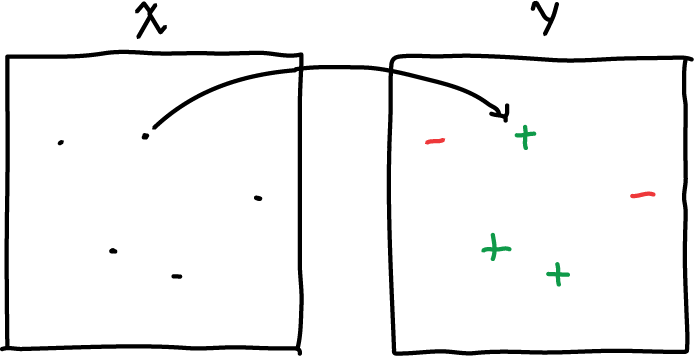
\includegraphics[width=.5\textwidth]{function}
    \caption{Um algoritmo genérico: $\mathcal{X} \to \mathcal{Y}$.}
    \label{fig:function}
\end{figure}

\begin{figure}[!htp]
    \centering
    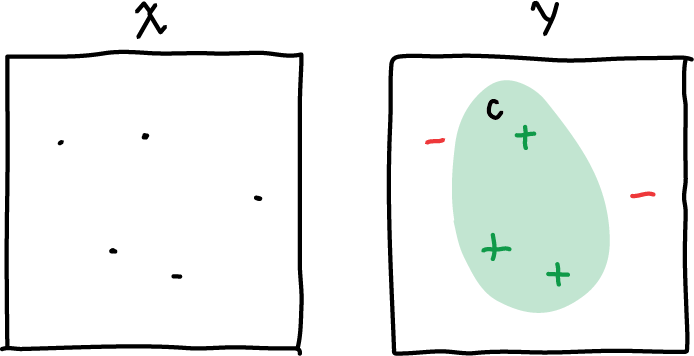
\includegraphics[width=.5\textwidth]{concept}
    \caption{Um conceito $c$.}
    \label{fig:concept}
\end{figure}

No contexto de aprendizado de máquina, não sabemos expressar essa função alvo, portanto teremos que inferi-la, aprendê-la. Chamaremos essa função ideal de \textbf{conceito} (figura \ref{fig:concept}). É o conceito que queremos aprender. No modelo PAC, um conceito é uma função $c: \mathcal{X} \to \{+,-\}$, ou seja, uma função que mapeia o espaço das instâncias em um valor \emph{booleano}.


\begin{figure}[!htp]
    \centering
    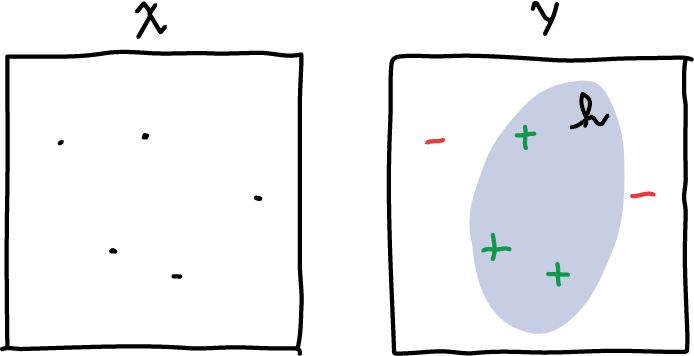
\includegraphics[width=.5\textwidth]{hypothesis}
    \caption{Uma hipótese $h \in \mathcal{H}$.}
    \label{fig:hypothesis}
\end{figure}


A função realmente obtida, a regra, a heurística, chamamos de \textbf{hipótese}(figura \ref{fig:hypothesis}). 

\begin{figure}[!htp]
    \centering
    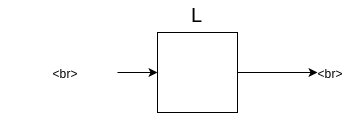
\includegraphics[width=.5\textwidth]{diagram}
    \caption{Um aprendiz genérico $L$.}
    \label{fig:diagram}
  \end{figure}


  \begin{figure}[!htp]
      \centering
      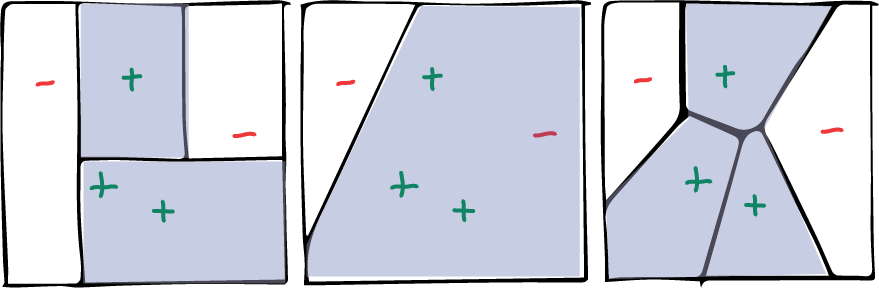
\includegraphics[width=.95\textwidth]{hspaces}
      \caption{hipóteses pertencentes a diferentes espaços de hipóteses $\mathcal{H}$.}
      \label{fig:hspaces}
  \end{figure}
O aprendiz (figura \ref{fig:diagram}), portanto, escolhe uma hipótese $h$
restrita às generalizações permitidas e preferidas pelo espaço de hipóteses $\mathcal{H}$ (figura \ref{fig:hspaces}).
\begin{figure}[!htp]
    \centering
    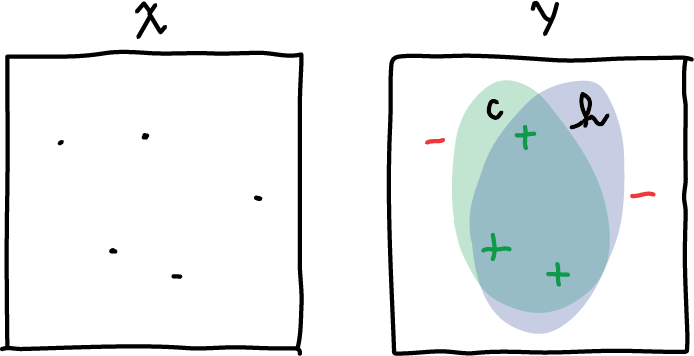
\includegraphics[width=.5\textwidth]{conceptVShypothesis}
    \caption{O erro, $c(x)\neq h(x)$} .
    \label{fig:erros}
\end{figure}
O objetivo do aprendiz $L$ é generalizar bem, ou seja,  escolher uma hipótese com menor erro na distribuição desconhecida $\mathcal{D}=P(\mathcal{X})$, menor \textbf{erro absoluto} ($erro_{\mathcal{D}}$). Entretanto, $L$ só tem conhecimento do \textbf{erro de treinamento}, $erro_{S}(h)$ (figura \ref{fig:erros}). Podemos formular o erro absoluto e o erro de treinamento da seguinte forma~\cite{MitchelPAC}:
\begin{equation}
    erro_{\mathcal{D}}(h) \equiv Pr_{x \sim \mathcal{D}}[c(x) \neq h(x)]
\end{equation}
\begin{equation}
  erro_{S}(h) \equiv Pr_{x \sim S}[c(x) \neq h(x)]
\end{equation}

\subsection{Objetivo}
O objetivo do \textbf{modelo PAC} é caracterizar a classe dos conceitos alvo que podem ser aprendidos de forma confiável em um número razoável de passos e amostras de treinamento.

\begin{equation}
    \underbrace{\text{ Provavelmente }}_{>(1-\delta)}
    \underbrace{\text{ Aproximadamente }}_{\leq\epsilon}
    \underbrace{\text{   Correto   }}_{\underset{x \sim \mathcal{D}}{Pr}[c(x) \neq h(x)]=0} \nonumber
  \end{equation}.

\bigskip

\noindent\fbox{%
    \parbox{\textwidth}{%
        $C$ é \textbf{PAC-apreensível} por $L$ se e somente se, com probabilidade $1 - \delta$, $L$ gera uma hipótese $h \in \mathcal{H}$ com $erro_{\mathcal{D}}(h)\leq\epsilon$ com número de amostras polinomial em função de $\rfrac{1}{\delta}$, $\rfrac{1}{\epsilon}$, $|\mathcal{X}|$ e $|\mathcal{H}|$, para $0 < \epsilon \leq \frac{1}{2}$ e $0 < \delta \leq \frac{1}{2}$.
    }%
  }
  
  \bigskip

  \noindent\fbox{%
  \parbox{\textwidth}{%
      $C$ é \textbf{eficientemente PAC-apreensível} por $L$ se e somente se $L$ é \textbf{PAC-apreensível} e gera hipótese em tempo polinomial em função de $\rfrac{1}{\delta}$, $\rfrac{1}{\epsilon}$, $|\mathcal{X}|$ e $|\mathcal{H}|$.
  }%
}

\bigskip

\subsection{Teorema de Haussler (1988): Limite do erro absoluto.}

Dado um certo algoritmo de aprendizado $L$, restrito ao seu  espaço de hipóteses $\mathcal{H}$, queremos saber a priori quantas amostras, $m$, serão necessárias para aprender um determinado conceito com determinada precisão. 

É disso que trata o teorema de Haussler\cite{Haussler1988}. Para um espaço de hipóteses finito e que contém o conceito que se quer aprender, ele dá um limite inferior no erro absoluto esperado dado um número de amostras $m$ ou no limite mínimo de amostras necessárias $m$ para um aprendiz consistente aprender o conceito $C$ com níveis aceitáveis de precisão e confiança.

\bigskip

\noindent\fbox{%
    \parbox{\textwidth}{%
    \textbf{Teorema: } Seja $\mathcal{H}$ finito. Seja $L$ um aprendiz que para qualquer conceito alvo $c$ e distribuição desconhecida $\mathcal{D}$ retorna uma hipótese consistente $h: erro_{S}(h)=0$. Seja $|S|=m, m \geq 1$, então \\
      $Pr[\exists h \in \mathcal{H}: error_{\mathcal{D}}(h)>\epsilon]\leq |H|e^{-\epsilon m}$
    }%
  }

  \begin{proof}  Sejam $h_i (i = 1, ..., k)$ todas as hipóteses em $\mathcal{H}$ tais que $erro_{\mathcal{D}}(h_i)>\epsilon$, temos:
    \begin{align}
        Pr_{x_j\sim\mathcal{S}}[(c(x_j) \neq h_i(x_j))=0] \leq (1-\epsilon) \label{haussler:a} \\
        Pr[\forall h \in |\mathcal{H}|: (erro_{S}(h)=0 \land erro_{\mathcal{D}}(h)> \epsilon)] \leq (1-\epsilon)^m \label{haussler:b} \\
        Pr[\exists h \in H: erro_{\mathcal{D}}(h)>\epsilon]\leq k (1-\epsilon)^m \label{haussler:c} \\
        Pr[\exists h \in H: erro_{\mathcal{D}}(h)>\epsilon]\leq |\mathcal{H}| (1-\epsilon)^m \label{haussler:d} \\ 
        (1-x) \leq e^{-x}, 0 \leq x \leq 1 \implies Pr[\exists h \in \mathcal{H}: error_{\mathcal{D}}(h)>\epsilon]\leq |H|e^{-\epsilon m}  \label{haussler:e} \\
        \qedhere
    \end{align}
    \end{proof}

A probabilidade de uma hipótese "ruim" ($erro_{\mathcal{D}}(h_i)>\epsilon$) prever corretamente uma determinada amostra é $\leq (1-\epsilon)$ (equação \ref{haussler:a}). Portanto, a probabilidade de uma hipótese "ruim" prever corretamente todas as amostras de treinamento é  $\leq (1-\epsilon)^m$ (equação \ref{haussler:b}). Há hipóteses "boas" e "ruins", imaginando que há $k$ hipóteses "ruins", a probabilidade de alguma destas $k$ hipóteses "ruins" prever corretamente todo o conjunto de treinamento é $\leq k (1-\epsilon)^m$ (equação \ref{haussler:c}). Como essas hipóteses "ruins" pertencem a $\mathcal{H}$, $k$ é necessariamente menor que $|\mathcal{H}|$, portanto chegamos ao limite do erro absoluto de $h$ dado uma precisão $\epsilon$  e um número de amostras $m$ (equação \ref{haussler:d}).

Como dito anteriormente, uma outra forma de ver o Teorema de Haussler é que para uma determinada tolerância ao erro $\epsilon$ e confiança $(1-\delta)$, o teorema dá o limite inferior no número de amostras de treinamento, $m \geq \frac{1}{\epsilon}(\ln{|\mathcal{H}|}+\ln{\frac{1}{\delta}})$,  para se aprender a classe de conceitos $C$.

\bigskip

\noindent\fbox{%
    \parbox{\textwidth}{%
    $|H|e^{-\epsilon m}=\delta \implies $ aprendiz $L$ aprende $C$ em $m = \frac{1}{\epsilon}(\ln{|\mathcal{H}|}+\ln{\frac{1}{\delta}})$ amostras de treinamento. 
    }%
}

\begin{proof}  Dado que o  Teorema de Haussler demonstra que $|\mathcal{H}|e^{-\epsilon m}$ é um limite inferior para a probabilidade do \textbf{erro absoluto} ultrapassar a tolerância ao erro ($\epsilon$) e que o modelo de aprendizado-PAC tem como limite inferior desta mesma probabilidade o valor $\delta$, podemos supor $|\mathcal{H}|e^{-\epsilon m}=\delta$, consequentemente:
\begin{align}
    |\mathcal{H}|e^{-\epsilon m}=\delta \implies e^{-\epsilon m} = \frac{\delta}{|\mathcal{H}|} \\
    - \epsilon m = (\ln{\delta} - \ln{|\mathcal{H}|})  \\
    \epsilon m = (\ln{|\mathcal{H}|} - \ln{\delta}) \\
    m = \frac{1}{\epsilon}(\ln{|\mathcal{H}|} + \ln{\frac{1}{\delta}}) \\
    \qedhere
\end{align}
\end{proof}


Interessante notar que esse limite inferior no número de amostras é idependente de $C$ ou $\mathcal{D}$ e logarítmico em relação ao tamanho do espaço $\mathcal{H}$~\cite{Haussler1988}.
% %------------------------------------------------

\section{Conclusão}

Teoria de Aprendizagem Computacional traz um arcabouço teórico que nos permite estimar o número de amostras de treinamento necessárias para um algoritmo convergir, com alta probabilidade, para uma boa generalização. 

Em particular, mostramos que para convergir com determinado nível de confiança e tolerância a erro, o limite inferior no tamanho do conjunto de treinamento é independente da classe de conceitos alvo ou da distribuição das instâncias de entrada e depende apenas logaritmicamente do tamanho do espaço de hipóteses. 

Na prática, no entanto, esses limites são muito "frouxos"\cite{MitchelPAC} e dão a falsa impressão que modelos mais simples (menor cardinalidade no espaço de hipóteses) são sempre melhores, o que não corresponde com a realidade em que modelos complexos e grandes como redes neurais profundas apresentam melhores generalizações para um grande número de aplicações.

%----------------------------------------------------------------------------------------
%	BIBLIOGRAPHY
%----------------------------------------------------------------------------------------

\renewcommand{\refname}{Referências} % Change the default bibliography title

\bibliography{references} % Input your bibliography file

%----------------------------------------------------------------------------------------

\end{document}